\RequirePackage{currfile}
\documentclass[12pt]{beamer}
\usepackage[utf8]{inputenc}
\usepackage[spanish]{babel}
\usepackage{standalone}
\usepackage{color}
\usepackage{siunitx}
\usepackage{hyperref}
%\hypersetup{colorlinks,linkcolor=,urlcolor=blue}
%\hypersetup{colorlinks,urlcolor=blue}
\usepackage{xcolor,soul}
\usepackage{etoolbox}
\usepackage{amsmath}
\usepackage{amsthm}
\usepackage{physics}
\usepackage{multicol}
\usepackage{bookmark}
\usepackage{longtable}
\usepackage{listings}
\usepackage{graphicx}
\usepackage{tikz}
\usetikzlibrary{patterns, matrix, backgrounds, decorations,shapes, arrows.meta}
\usepackage[autostyle,spanish=mexican]{csquotes}
\usepackage[os=win]{menukeys}
\usepackage{pifont}
\usepackage{pbox}
\usepackage{caption}
\captionsetup{font=scriptsize,labelfont=scriptsize}
%\usepackage[sfdefault]{roboto}  %% Option 'sfdefault' only if the base font of the document is to be sans serif

%Sección de definición de colores
\definecolor{ao}{rgb}{0.0, 0.5, 0.0}
\definecolor{bisque}{rgb}{1.0, 0.89, 0.77}
\definecolor{amber}{rgb}{1.0, 0.75, 0.0}
\definecolor{armygreen}{rgb}{0.29, 0.33, 0.13}
\definecolor{alizarin}{rgb}{0.82, 0.1, 0.26}
\definecolor{cadetblue}{rgb}{0.37, 0.62, 0.63}
\definecolor{deepblue}{rgb}{0,0,0.5}
\definecolor{brown}{rgb}{0.59, 0.29, 0.0}
\definecolor{OliveGreen}{rgb}{0,0.25,0}


\usefonttheme[onlymath]{serif}
%Sección de definición de nuevos comandos

\newcommand*{\TitleParbox}[1]{\parbox[c]{1.75cm}{\raggedright #1}}%
\newcommand{\python}{\texttt{python}}
\newcommand{\textoazul}[1]{\textcolor{blue}{#1}}
\newcommand{\azulfuerte}[1]{\textcolor{blue}{\textbf{#1}}}
\newcommand{\funcionazul}[1]{\textcolor{blue}{\textbf{\texttt{#1}}}}
\newcommand{\ptilde}[1]{\ensuremath{{#1}^{\prime}}}
\newcommand{\stilde}[1]{\ensuremath{{#1}^{\prime \prime}}}
\newcommand{\ttilde}[1]{\ensuremath{{#1}^{\prime \prime \prime}}}
\newcommand{\ntilde}[2]{\ensuremath{{#1}^{(#2)}}}
\renewcommand{\arraystretch}{1.5}

\newcounter{saveenumi}
\newcommand{\seti}{\setcounter{saveenumi}{\value{enumi}}}
\newcommand{\conti}{\setcounter{enumi}{\value{saveenumi}}}
\renewcommand{\rmdefault}{cmr}% cmr = Computer Modern Roman

\linespread{1.5}

\usefonttheme{professionalfonts}
%\usefonttheme{serif}
\DeclareGraphicsExtensions{.pdf,.png,.jpg}


%Sección para el tema de beamer, con el theme, usercolortheme y sección de footers
\mode<presentation>
{
  \usetheme{Warsaw}
  
  %\useoutertheme{infolines}
  \useoutertheme{default}
  \usecolortheme{spruce}
  \setbeamercovered{invisible}
  % or whatever (possibly just delete it)
  \setbeamertemplate{section in toc}[sections numbered]
  \setbeamertemplate{subsection in toc}[subsections numbered]
  \setbeamertemplate{subsection in toc}{\leavevmode\leftskip=3.2em\rlap{\hskip-2em\inserttocsectionnumber.\inserttocsubsectionnumber}\inserttocsubsection\par}
  \setbeamercolor{section in toc}{fg=blue}
  \setbeamercolor{subsection in toc}{fg=blue}
  \setbeamercolor{frametitle}{fg=blue}
  \setbeamertemplate{caption}[numbered]

  \setbeamertemplate{footline}
  \beamertemplatenavigationsymbolsempty
  \setbeamertemplate{headline}{}
}

\makeatletter
\setbeamercolor{section in foot}{bg=gray!30, fg=black!90!orange}
\setbeamercolor{subsection in foot}{bg=blue!30!yellow, fg=red}
\setbeamertemplate{footline}
{
  \leavevmode%
  \hbox{%
  \begin{beamercolorbox}[wd=.333333\paperwidth,ht=2.25ex,dp=1ex,center]{section in foot}%
    \usebeamerfont{section in foot} \insertsection
  \end{beamercolorbox}}%
  \begin{beamercolorbox}[wd=.333333\paperwidth,ht=2.25ex,dp=1ex,center]{subsection in foot}%
    \usebeamerfont{subsection in foot}  \insertsubsection
  \end{beamercolorbox}%
  \begin{beamercolorbox}[wd=.333333\paperwidth,ht=2.25ex,dp=1ex,right]{date in head/foot}%
    \usebeamerfont{date in head/foot} \insertshortdate{} \hspace*{2em}
    \insertframenumber{} / \inserttotalframenumber \hspace*{2ex} 
  \end{beamercolorbox}}%
  \vskip0pt%
\makeatother  

\makeatletter
\patchcmd{\beamer@sectionintoc}
  {\vfill}
  {\vskip\itemsep}
  {}
  {}
\makeatother


\title{\large{Funciones Gamma y Beta}}
\subtitle{Tema 1 - La física y la geometría}
\author{M. en C. Gustavo Contreras Mayén}
\date{\today}
\institute{Facultad de Ciencias - UNAM}
\titlegraphic{
\includegraphics[width=1.75cm]{../Imagenes/escudo-facultad-ciencias}\hspace*{4.75cm}~%
   
\includegraphics[width=1.75cm]{../Imagenes/escudo-unam}
}
\setbeamertemplate{navigation symbols}{}
\begin{document}
\maketitle
\fontsize{14}{14}\selectfont
\spanishdecimal{.}
\section*{Contenido}
\frame[allowframebreaks]{\tableofcontents[currentsection, hideallsubsections]}
\section{Introducción}
\frame[allowframebreaks]{\tableofcontents[currentsection, hideothersubsections]}
\subsection{Integrales como funciones}
\begin{frame}
\frametitle{Integrales como funciones}
Las integrales son uno de los medios matemáticos más convenientes con los que se pueden definir nuevas funciones.
\\
\bigskip
Si el integrando o los límites de integración incluyen parámetros, esos parámetros pueden tratarse como variables y la integral misma como una función de esos parámetros.
\end{frame}
\begin{frame}
\frametitle{Integrales como funciones}
Haremos una revisión de algunas funciones más importantes que normalmente se definen en términos de integrales.
\end{frame}
\subsection{Funciones de apoyo}
\begin{frame}
\frametitle{Utilidad de las funciones $\Gamma$ y $B$}
La función Gamma $\Gamma$ aparece ocasionalmente en problemas de física tales como:
\setbeamercolor{item projected}{bg=blue!70!black,fg=yellow}
\setbeamertemplate{enumerate items}[circle]
\begin{enumerate}[<+->]
\item Cálculo de probabilidades en mecánica estadística.
\item La normalización de las funciones de onda para el potencial de Coulomb en Mecánica Cuántica.
\end{enumerate}
\end{frame}
\begin{frame}
\frametitle{Utilidad de las funciones $\Gamma$ y $B$}
En realidad la función $\Gamma$ tiene pocas aplicaciones directas en física, sin embargo es importante porque nos permite desarrollar otras funciones que si tienen una aplicación directa en la física, como por ejemplo: las funciones de Bessel.
\end{frame}
\begin{frame}
\frametitle{Utilidad de las funciones $\Gamma$ y $B$}
La relación entre las funciones $\Gamma$ y $B$ también nos permitirán expresar de manera más compacta los resultados que se obtendrán al resolver ciertas ecuaciones diferenciales que veremos a lo largo del curso.
\end{frame}
\begin{frame}
\frametitle{Utilidad de las funciones $\Gamma$ y $B$}
Es por ello que al manejar debidamente estas funciones (y sus variantes), tendremos más herramientas para nuestro objetivo: resolver un problema de la física mediante el uso de funciones especiales, y con ello, interpretar el fenómeno que estudiamos.
\end{frame}
\begin{frame}
\frametitle{Nota importante}
Para el manejo de estas funciones será necesario un trabajo fluido en cuanto a la solución de integrales tanto definidas como indefinidas, por lo que tendrás oportunidad de ejercitar lo aprendido en los cursos de cálculo.
\end{frame}
\begin{frame}
\frametitle{Nota importante}
Es cierto que existe software matemático (Wolfram, Mathematica, etc.) que te devolverá la solución para algunas integrales, pero confiamos en que utilizarás esas herramientas para corroborar tus resultados, es decir, esperamos que resuelvas \enquote{a mano} cada una de las integrales que se te presenten.
\end{frame}
\begin{frame}
\frametitle{Nota importante}
Recuerda que es necesario contar con la evidencia de tu trabajo en la solución de un ejercicio, así que como diría un maestro: \enquote{hay que arrastrar el lápiz}.
\end{frame}
% Referencia: Boas (2005) Chap. 11 Special Functions
\section{La función factorial}
\frame[allowframebreaks]{\tableofcontents[currentsection, hideothersubsections]}
\subsection{Definición}
\begin{frame}
\frametitle{Construcción}
Calculemos el valor de la siguiente integral, para $\alpha > 0$:
\begin{align}
\int_{0}^{\infty} e^{-\alpha \, x} \dd{x} = - \dfrac{1}{\alpha} e^{-\alpha \, x}\eval_{0}^{\infty} = \dfrac{1}{\alpha}
\label{eq:ecuacion_02_01}
\end{align}
\pause
\fontsize{12}{12}\selectfont
\begin{block}{Nota importante}
Con el fin de mantener una buena legibilidad, escribiremos el argumento de la función exponencial como superíndice $e^{-\alpha \, x}$, pero si el argumento es extenso, la función se escribirá como $\exp(-\alpha \, x)$
\end{block}
\end{frame}
\begin{frame}
\frametitle{Construcción}
Diferenciamos con respecto a $\alpha$ ambos lados de la ec. (\ref{eq:ecuacion_02_01}):
\begin{align*}
\int_{0}^{\infty} - x \, e^{-\alpha \, x} \dd{x} = - \dfrac{1}{\alpha^{2}} &= \int_{0}^{\infty} x \, e^{-\alpha \, x} \dd{x} = \dfrac{1}{\alpha^{2}} \\[0.5em]
&= \int_{0}^{\infty} x^{2} \, e^{-\alpha \, x} \dd{x} = \dfrac{2}{\alpha^{3}} \\[0.5em]
&= \int_{0}^{\infty} x^{3} \, e^{-\alpha \, x} \dd{x} = \dfrac{3!}{\alpha^{4}} \\
& \vdots
\end{align*}
\end{frame}
\begin{frame}
\frametitle{La expresión general}
La expresión general luego de $n$ pasos de diferenciación con respecto a $\alpha$ es:
\begin{align}
\int_{0}^{\infty} x^{n} \, e^{-\alpha \, x} \dd{x} = \dfrac{n!}{\alpha^{n+1}}
\label{eq:ecuacion_02_02}
\end{align}
\end{frame}
\begin{frame}
\frametitle{Caso especial}
Haciendo que $\alpha = 1$, se obtiene
\begin{align}
\int_{0}^{\infty} x^{n} \, e^{-\alpha \, x} \dd{x} = n! \hspace{1cm} n = 1, 2, 3, \ldots
\label{eq:ecuacion_02_03}
\end{align}
\pause
Así tenemos una integral definida cuyo valor es $n!$ para un entero positivo $n$.
\end{frame}
\begin{frame}
\frametitle{Caso especial 2}
Usando la ec. (\ref{eq:ecuacion_02_03}) le podemos dar un significado al valor de $0!$: si hacemos $n = 0$, ocurre:
\begin{align}
0! = \int_{0}^{\infty} e^{-x} \dd{x} = -e^{x}\eval_{0}^{\infty} = 1
\label{eq:ecuacion_02_04}
\end{align}
\end{frame}
\section{Doble factorial}
\frame[allowframebreaks]{\tableofcontents[currentsection, hideothersubsections]}
\subsection{Notación}
\begin{frame}
\frametitle{Notación doble factorial}
En varios problemas de la física, en particular con los \emph{polinomios de Legendre}, encontraremos productos de enteros impares positivos y de pares positivos, por conveniencia, definimos el doble factorial:
\begin{align}
\begin{aligned}
1 \cdot 3 \cdot 5 \cdots (2 \, n+1) &= (2 \, n+1) !! \\
2 \cdot 4 \cdot 6 \cdots (2 \, n) &= (2 \, n) !!
\end{aligned}
\label{eq:ecuacion_10_33b}
\end{align}
\end{frame}
\begin{frame}
\frametitle{Notación doble factorial}
Que están relacionados con la función factorial
\begin{align}
\begin{aligned}
(2 \, n)!! &=  2^{n} \: n! \\[1em]
(2 \, n+1)!! &= \dfrac{(2 \, n+1)!}{2^{n} \, n!}
\end{aligned}
\label{eq:ecuacion_10_33c}
\end{align}
También se define $(-1)!! = 1$, un caso especial que no se obtiene de la ec. (\ref{eq:ecuacion_10_33c})
\end{frame}
\section{Función Gamma}
\frame[allowframebreaks]{\tableofcontents[currentsection, hideothersubsections]}
\subsection{Definición}
\begin{frame}
\frametitle{Definición función Gamma}
En el desarrollo que hemos hecho, $n$ es un número entero no negativo, es natural definir la función factorial para un $n$ no entero mediante la integral de la ec.(\ref{eq:ecuacion_02_03}).
\\
\bigskip
\pause
No hay ninguna objeción en la notación $n!$ para $n$ no entero, pero es habitual reservar la notación factorial para $n$ entero.
\end{frame}
\begin{frame}
\frametitle{Definición función Gamma}
Para el caso de una función para evaluar el factorial de un $n$ no entero, entonces llamaremos a esa función: la función gamma $(\Gamma)$.
\\
\bigskip
\pause
También es una práctica bastante común reemplazar $n$ por la letra $p$ cuando queremos decir que no es necesariamente un número entero.
\end{frame}
\begin{frame}
\frametitle{Definición función Gamma}
Siguiendo estas convenciones, se define la función Gamma para cualquier $p > 0$:
\begin{align}\addtolength{\fboxsep}{5pt}\boxed{
\Gamma (p) = \int_{0}^{\infty} x^{p-1} \, e^{-x} \dd{x}, \hspace{1cm} p > 0}
\label{eq:ecuacion_03_01}
\end{align}
\end{frame}
\begin{frame}
\frametitle{Puntos importantes}
\setbeamercolor{item projected}{bg=blue!70!black,fg=yellow}
\setbeamertemplate{enumerate items}[circle]
\begin{enumerate}[<+->]
\item Para $0 < p < 1$ la integral (\ref{eq:ecuacion_03_01}) se hace impropia, ya que el término $x^{p-1}$ tiende a infinito en el límite inferior.
\item Para $p > 0$ se tiene una integral que converge.
\item Para $p \leq 0$ la integral diverge y no se puede usar para definir $\Gamma (p)$, más adelante veremos cómo definir  $\Gamma (p)$ para $p \leq 0$.
\end{enumerate}
\end{frame}
\subsection{Primeras propiedades}
\begin{frame}
\frametitle{Primeras propiedades}
De las ecs. (\ref{eq:ecuacion_03_01}) y (\ref{eq:ecuacion_02_03}), se tiene que:
\begin{align}
\begin{aligned}
\Gamma (n) &= \int_{0}^{\infty} x^{n-1} \, e^{-x} \dd{x} = (n -1)! \\[1em]
\Gamma (n+1) &= \int_{0}^{\infty} x^{n} \, e^{-x} \dd{x} = n!
\end{aligned}
\label{eq:ecuacion_03_02}
\end{align}
\end{frame}
\begin{frame}
\frametitle{Resultado}
Entonces:
\\
\begin{minipage}{0.3\linewidth}
\begin{align*}
\Gamma (1) &= 0! = 1 \\
\Gamma (2) &= 1! = 1 \\
\Gamma (3) &= 2! = 2 \\
\Gamma (4) &= 3! = 6 \\
&\ldots \\
\Gamma (n) &= n-1!
\end{align*}
\end{minipage}
\hspace{0.7cm}
\pause
\begin{minipage}{0.5\linewidth}
Donde el factorial de un entero positivo $n$, es el que conocemos del álgebra.
\end{minipage}
\end{frame}
\begin{frame}
\frametitle{Función Gamma para $p+1$}
Al reemplazar $p$ por $p+1$ en la ec. (\ref{eq:ecuacion_03_01}) nos deja:
\begin{align}
\Gamma (p+1) = \int_{0}^{\infty} x^{p} \, e^{-x} \dd{x} = p!, \hspace{1cm} p > -1
\label{eq:ecuacion_03_03}
\end{align}
\pause
En algunos textos se ocupa la notaciona factorial $p! = \Gamma (p+1)$, aunque $p$ es un no entero.
\end{frame}
\subsection{Relación de recurrencia}
\begin{frame}
\frametitle{Resolviendo la integral}
Al integrar por partes la ec. (\ref{eq:ecuacion_03_03}), haciendo
\begin{align*}
x^{p} =  u \hspace{2cm} e^{-x} \dd{x} =  \dd{v}
\end{align*}
\pause
Entonces tenemos que
\begin{eqnarray*}
\dd{u} &= p \, x^{p-1} \dd{x}, \hspace{1cm} v = - e^{-x} \\[1em]
\pause
\Gamma (p+1) &= -x^{p} \, e^{-x} \displaystyle \eval_{0}^{\infty} - \displaystyle \int_{0}^{\infty} \left(-e^{-x} \right) \, p \, x^{p-1} \dd{x} = \\[1em]
\pause
&= p \displaystyle \int_{0}^{\infty} x^{p-1} \, e^{-x} \dd{x}
\end{eqnarray*}
\end{frame}
\begin{frame}
\frametitle{Resolviendo la integral}
Donde reconocemos la integral que define a la función Gamma, entonces obtenemos la regla de recurrencia:  
\begin{align}
\boxed{\Gamma (p+1) = p \, \Gamma (p)}
\label{eq:ecuacion_03_04}
\end{align}
Es de utilidad para simplificar expresiones que involucran a la función $\Gamma$.
\end{frame}
\subsection{Función Gamma para \texorpdfstring{$p < 0$}{p < 0}}
\begin{frame}
\frametitle{Función Gamma para $p < 0$}
Para valores $p < 0$, la función $\Gamma (p)$ no se ha definido hasta el momento.
\\
\bigskip
\pause
Ocuparemos la relación de recursividad ec. (\ref{eq:ecuacion_03_04}) para resolverla.
\end{frame}
\begin{frame}
\frametitle{Función Gamma para $p < 0$}
Entonces:
\begin{align}
\boxed{\Gamma (p) = \dfrac{1}{p} \, \Gamma (p + 1)}
\label{eq:ecuacion_04_01}
\end{align}
que define la función $\Gamma$ para valores $p < 0$
\end{frame}
\begin{frame}
\frametitle{Ejemplos}
Veamos un par de ejemplos: 
\setbeamercolor{item projected}{bg=blue!70!black,fg=yellow}
\setbeamertemplate{enumerate items}[circle]
\begin{enumerate}[<+->]
\item  Se quiere obtener el valor de $\Gamma (-0.3)$, entonces podemos resolverlo de la siguiente manera:
\begin{align*}
\Gamma (-0.3) = - \dfrac{1}{0.3} \, \Gamma (0.7)
\end{align*}
\seti
\end{enumerate}
\end{frame}
\begin{frame}
\frametitle{Ejemplos}
\setbeamercolor{item projected}{bg=blue!70!black,fg=yellow}
\setbeamertemplate{enumerate items}[circle]
\begin{enumerate}[<+->]
\conti
\item  Se quiere obtener el valor de $\Gamma (-0.3)$, entonces podemos resolverlo de la siguiente manera:
\begin{align*}
\Gamma (-1.3) = - \dfrac{1}{(-1.3)(-0.3)} \, \Gamma (0.7)
\end{align*}
\end{enumerate}
\fontsize{12}{12}\selectfont
Los valores de la función $\Gamma$ se pueden obtener de tablas, pero lo más práctico es ocupar el software matemático (Wolfram, Mathematica) o lenguajes de programación que incluyen librerías científicas, como \python.
\end{frame}
\begin{frame}
\frametitle{El caso de enteros negativos}
De este y el uso sucesivo de la ec. (\ref{eq:ecuacion_04_01}) se deduce que la función $\Gamma (p)$ tiende a infinito no solo en cero sino también en todos los enteros negativos.
\\
\bigskip
\pause
En los intervalos entre los enteros negativos, alterna valores positivos y negativos, negativo de 0 a -1, positivo de -1 a -2, y así sucesivamente, como puede ver en la siguiente figura (\ref{fig:figura_plot_gamma}).
\end{frame}
\begin{frame}
\frametitle{Gráfica de $\Gamma (p)$}
\begin{figure}[h!]
   \centering
   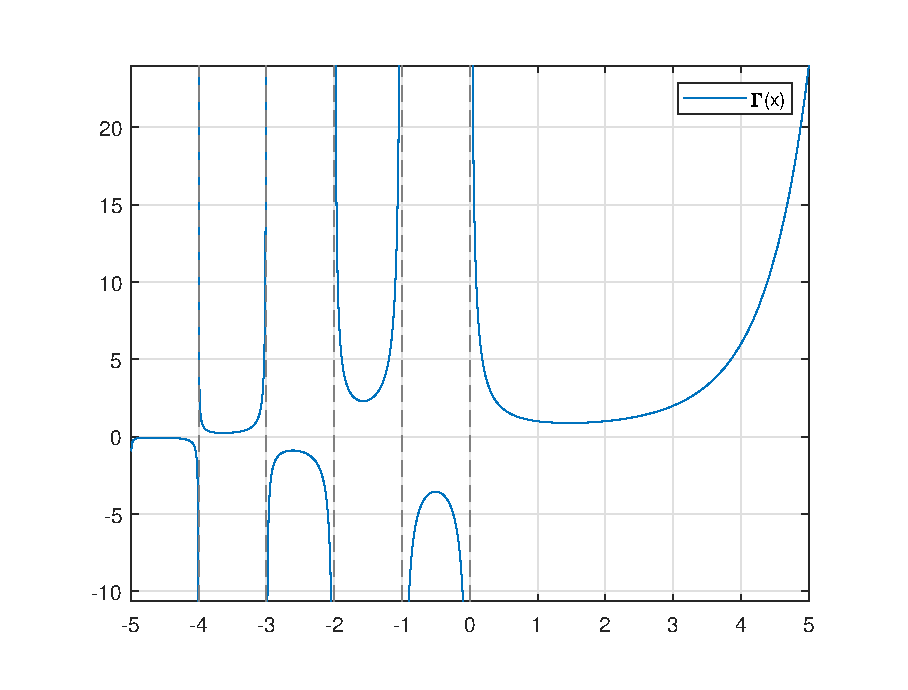
\includegraphics[scale=0.55]{Imagenes/Plot_Gamma.eps}
   \caption{Gráfica de la función Gamma $\Gamma (p)$}
   \label{fig:figura_plot_gamma}
\end{figure}
\end{frame}
\section{Fórmulas que involucran a \texorpdfstring{$\Gamma (p)$}{}}
\frame[allowframebreaks]{\tableofcontents[currentsection, hideothersubsections]}
\subsection{Algunas fórmulas}
\begin{frame}
\frametitle{Aclaración importante}
Como veremos a continuación, el desarrollo de las fórmulas para la función $\Gamma (p)$, se sigue de la definición, por lo que la operación algebraica y de solución de la integral es completamente posible.
\end{frame}
\begin{frame}
   \frametitle{Aclaración importante}
Nos interesa que dispongan de una relación de fórmulas y que puedan ocuparlas en donde sea necesario.
\\
\bigskip
Aunque las fórmulas son válidas, en el caso que se indique, deberán de demostrar la fórmula que vayan a utilizar.
\end{frame}
\begin{frame}
\frametitle{Una fórmula importante}
Evaluemos $\Gamma (1/2)$. Usando la definición:
\begin{align}
\Gamma \left( \dfrac{1}{2}\right) = \int_{0}^{\infty} \dfrac{1}{\sqrt{t}} \, e^{-t} \dd{t}
\label{eq:ecuacion_05_01}
\end{align}
\pause
Toma en cuenta que no importa qué letra usemos para la variable \enquote{muda} de integración en una integral definida.
\end{frame}
\begin{frame}
\frametitle{Resolviendo la integral}
Haciendo el cambio de variable en la ec. (\ref{eq:ecuacion_05_01}):
\begin{align*}
t = y^{2} \hspace{0.5cm} \Rightarrow \dd{t} = 2 \, y \dd{y}
\end{align*}
Entonces tenemos que
\begin{align*}
\Gamma \left( \dfrac{1}{2} \right) = \int_{0}^{\infty} \, e^{-y^{2}} \, 2 \, y \dd{y} = 2 \int_{0}^{\infty} \, e^{-y^{2}} \dd{y}
\end{align*}
\fontsize{12}{12}\selectfont
\end{frame}
\begin{frame}
\frametitle{Resolviendo la integral}
Con $x$ como la variable \enquote{muda} de integración:
\begin{align}
\Gamma \left( \dfrac{1}{2} \right) = 2 \int_{0}^{\infty} \, e^{-x^{2}} \dd{x}
\label{eq:ecuacion_05_02}
\end{align}
\pause
Multiplicando las dos integrales de $\Gamma (1/2)$ para luego escribir el resultado como una integral doble:
\begin{align*}
\left[ \Gamma \left( \dfrac{1}{2} \right) \right]^{2} = 4 \int_{0}^{\infty} \, \int_{0}^{\infty} \, e^{-(x^{2} + y^{2}} \dd{x} \dd{y}
\end{align*}
\end{frame}
\begin{frame}
\frametitle{Resolviendo la integral}
Tenemos una doble integral sobre el primer cuadrante de una circunferencia, por lo que es más fácil evaluarla en coordenadas polares:
\begin{align*}
\left[ \Gamma \left( \dfrac{1}{2} \right) \right]^{2} &= 4 \int_{0}^{\pi/2} \, \int_{0}^{\infty} \, e^{-r^{2}} \, r \dd{r} \dd{\theta} = \\[0.5em]
&= 4 \, \dfrac{\pi}{2} \, \dfrac{e^{-r^{2}}}{-2}\eval_{0}^{\infty} = \\[0.5em]
&= \pi
\end{align*}
\end{frame}
\begin{frame}
\frametitle{Primera fórmula}
Entonces obtenemos la primera fórmula:
\begin{align}
\boxed{\Gamma \left( \dfrac{1}{2} \right) = \sqrt{\pi}}
\label{eq:ecuacion_05_03}
\end{align}
\end{frame}
\subsection{Otras fórmulas}
\begin{frame}
\frametitle{Otras fórmulas para $\Gamma(p)$}
A continuación se enlistan algunas de las fórmulas que involucran a la función Gamma, toma en cuenta de que a pesar de que no se demuestra la expresión, en el caso de que la utilices para un ejercicio, deberás de presentar la respectiva demostración.
\end{frame}
\begin{frame}
\frametitle{Otras fórmulas para $\Gamma(x)$}
\fontsize{12}{12}\selectfont
\begin{align*}
\Gamma (x) &= (x - 1) \, \Gamma(x - 1) \hspace{1cm} x \neq 0, -1, -2, \ldots \\[0.75em]
\Gamma (-x) &= \dfrac{\Gamma (1- x)}{-x} \hspace{1cm} x \neq 0, 1, 2, \ldots \\[0.75em]
\Gamma (x) \, \Gamma (1 - x) &= \dfrac{\pi}{\sin x \, \pi}, \hspace{1.5cm} x \neq 0, \pm 1, \pm 2, \pm 3, \ldots \\[0.75em]
n! &= \left( \dfrac{n}{e} \right)^{n} \, \sqrt{2 \, \pi \, n} + h \\[0.5em]
&\mbox{con } n = 1, 2, 3, \ldots, \hspace{0.5cm} 0 < \dfrac{h}{n!} < \dfrac{1}{12 \, n}
\end{align*}
\end{frame}
\begin{frame}
\frametitle{Otras fórmulas para $\Gamma(x)$}
\fontsize{12}{12}\selectfont
\begin{align*}
\Gamma \left(n + \dfrac{1}{2} \right) &= \dfrac{1 \cdot 3 \cdot 5 \ldots (2 \, n - 1)\sqrt{\pi}}{2^{n}}, \hspace{0.7cm} n = 1, 2, 3, \ldots \\[0.75em]
\int_{0}^{\infty} t^{a} \, e^{-b \, t^{c}} \dd{t} &= \dfrac{\Gamma \left(\dfrac{a + 1}{c} \right)}{c \, b^{(a+1)/c}}, \\[0.5em]
&\mbox{con } a > -1, \hspace{0.5cm} b > 0, \hspace{0.5cm} c > 0   
\end{align*}
\end{frame}
\section{Función Beta}
\frame[allowframebreaks]{\tableofcontents[currentsection, hideothersubsections]}
\subsection{Definición}
\begin{frame}[fragile]
\frametitle{Definición de la función Beta}
La función Beta se define por la siguiente integral:
\begin{align} \addtolength{\fboxsep}{5pt}\boxed{
\begin{gathered}
B(p, q) = \int_{0}^{1} x^{p-1} \, (1- x )^{q-1} \dd{x}, \\
\mbox{con }  p > 0, q > 0
\end{gathered}
}
\label{eq:ecuacion_06_01}
\end{align}
\pause
Existen una serie de fórmulas para la función Beta que es conveniente conocer, todas ellas derivadas de la definición.
\end{frame}
\begin{frame}
\frametitle{Fórmulas para $B(p, q)$}
Si cambiamos el rango de integración de la ec. (\ref{eq:ecuacion_06_01}), haciendo $x = y/a$, entonces $x = 1$ corresponde a $y = a$, por lo que tenemos:
\begin{align} \addtolength{\fboxsep}{5pt}\boxed{
\begin{aligned}
B (p, q) &= \int_{0}^{a} \left( \dfrac{y}{a}\right)^{p-1} \, \left( 1 - \dfrac{y}{a}\right)^{q-1} \dfrac{\dd{y}}{a} \\[0.5em]
&= \dfrac{1}{a^{p+q-1}} \int_{0}^{a} y^{p-1} \, (a - y)^{q-1} \dd{y}
\end{aligned}
\label{eq:ecuacion_06_03}
}
\end{align}
\end{frame}
\subsection{Fórmula trigonométrica de \texorpdfstring{$B(p,q)$}{B(p, q)}}
\begin{frame}
\frametitle{Fórmula trigonométrica de $B(p,q)$}
Para obtener la forma trigonométrica de la función Beta, hacemos el cambio de variable $x = \sin^{2} \theta$, así
\begin{align*}
\dd{x} &= 2 \, \sin \theta \, \cos \theta \dd{\theta} \\[1em]
(1 - x) &= 1 - \sin^{2} \theta = \cos^{2} \theta \\[1em]
x &= 1 \hspace{0.3cm} \Rightarrow \hspace{0.3cm} \theta = \pi/2
\end{align*}
\end{frame}
\begin{frame}
\frametitle{Fórmula trigonométrica de $B(p, q)$}
Haciendo las sustituciones en la ec. (\ref{eq:ecuacion_06_01}):
{\fontsize{12}{12}\selectfont
\begin{align}
B(p, q) = \int_{0}^{\pi/2} \left( \sin^{2} \theta \right)^{p-1} \, \left( \cos^{2} \theta \right)^{q-1} \, 2 \, \sin \theta \, \cos \theta \dd{\theta}
\end{align}}
\pause
Simplificando la expresión llegamos a:
{\fontsize{12}{12}\selectfont
\begin{align}
\addtolength{\fboxsep}{5pt}\boxed{B(p, q) = 2 \, \int_{0}^{\pi/2} \left( \sin^{2} \theta \right)^{2p-1} \, \left( \cos^{2} \theta \right)^{2q-1} \dd{\theta}}
\label{eq:ecuacion_06_04}
\end{align}}
\end{frame}
\begin{frame}
\frametitle{Otra fórmula para $B(p, q)$}
Con el cambio de variable en la ec. (\ref{eq:ecuacion_06_01})
\begin{align*}
x = \dfrac{y}{(1 + y)}
\end{align*}
\pause
Se puede demostrar que
\begin{align}
\addtolength{\fboxsep}{5pt}\boxed{B(p, q) = \int_{0}^{\infty} \dfrac{y^{p-1}}{(1 + y)^{p+q}} \dd{y}}
\label{eq:ecuacion_06_05}
\end{align}   
\end{frame}
\begin{frame}
\frametitle{Otras fórmulas}
Como en el caso de la función $\Gamma (x)$, las fórmulas que se presentan para $B(p, q)$ se demuestran a partir de la definición y de un manejo algebraico, por lo que en caso de que utilices alguna en la solución de un ejercicio, tendrás que demostrar la fórmula.
\end{frame}
\begin{frame}
\frametitle{Otras fórmulas}
\begin{align*}
B (x, y) &= B (y, x) \\[1em]
B (x, 2-x) &= \dfrac{\pi}{\sin x \, \pi}, \hspace{1.5cm} 0 < x < 1   
\end{align*}
\end{frame}
\subsection{La funión Beta en términos de Gamma}
\begin{frame}
\frametitle{La función $B(p, q)$ en términos de $\Gamma (p)$}
La función Beta se expresa en términos de la función Gamma de la siguiente manera:
\begin{align}
\addtolength{\fboxsep}{5pt}\boxed{B(p, q) = \dfrac{\Gamma(p) \, \Gamma(q)}{\Gamma (p + q)}}
\label{eq:ecuacion_07_01}
\end{align}
Esta fórmula nos ayuda a evaluar una función $B (p, q)$ en términos de funciones $\Gamma$. \textbf{Nota: } también es fácil demostrar la expresión, para que en el caso de que la utilices, realices el ejercicio.
\end{frame}
\section{Ejemplos}
\frame[allowframebreaks]{\tableofcontents[currentsection, hideothersubsections]}
%Referencia: Farrell - Solved Problems in Analysis as Applied to Gamma Function II-39
\subsection{Longitud de una lemniscata}
\begin{frame}
\frametitle{Longitud de una leminiscata}
Usando la función Gamma, calcula la longitud de la lemniscata
\begin{align*}
\rho^{2} = a^{2} \, \cos 2 \theta
\end{align*}
\end{frame}
\begin{frame}
\frametitle{Longitud de una leminiscata}
\begin{wrapfigure}{r}{0.55\textwidth}
    \centering
    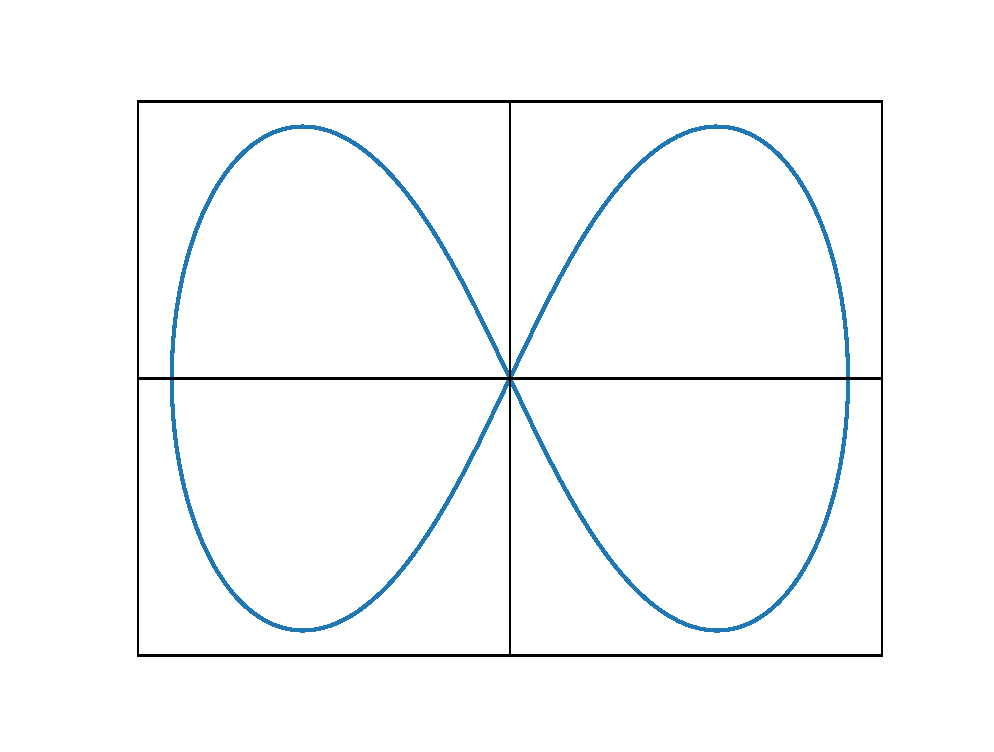
\includegraphics[scale=0.35]{Imagenes/plot_leminscata_01.eps}
    \caption{Gráfica de la lemniscata.}
    \label{fig:figura_lemniscata}
\end{wrapfigure}
La curva se parece a un ocho invertido, teniendo al eje x como eje de simetría, pasa en dos ocasiones por el origen, como se puede ver en la figura (\ref{fig:figura_lemniscata})
\end{frame}
\begin{frame}
\frametitle{Tomando la simetría del problema}
Para esta curva, por simetría se tiene la misma longitud en cada uno de los cuatro cuadrantes, por lo que podemos calcular la longitud en el primer cuadrante y luego multiplicarla por cuatro.
\end{frame}
\begin{frame}
\frametitle{Tomando la simetría del problema}
Los puntos donde la curva cruza el eje $x$ en el origen son aquellos para los cuales el argumento del coseno es un múltiplo entero, impar de $\pi / 2$. 
\\
\bigskip
Para el tramo en el primer cuadrante, tomamos $0 \leq \theta \leq \pi/4$.
\end{frame}
\begin{frame}
\frametitle{Resolviendo el problema}
La longitud de la curva en coordenadas polares es
\begin{align*}
s = \int_{\alpha}^{\beta} \left[ \rho^{2} + \left( \dv{\rho}{\theta} \right)^{2} \right]^{1/2} \dd{\theta}
\end{align*}
\pause
Como $\rho^{2} = a^{2} \, \cos 2 \theta$, tenemos que:
\begin{align*}
\left( \dv{\rho}{\theta} \right)^{2} = \dfrac{a^{4} \, \sin^{2} 2 \theta}{a^{2} \, \cos 2 \theta}
\end{align*}
\end{frame}
\begin{frame}
\frametitle{Resolviendo el problema}
Entonces:
\begin{align*}
\dfrac{1}{4} \, s &= \int_{0}^{\pi/4} \left( a^{2} \, \cos 2 \theta + \dfrac{a^{4} \, \sin^{2} 2 \theta}{\cos 2 \theta} \right)^{1/2} \dd{\theta} = \\[1em]
&= \int_{0}^{\pi/4} a \, \cos^{-1/2} 2 \theta \dd{\theta}
\end{align*}
\end{frame}
\begin{frame}
\frametitle{Resolviendo al integral}
Haciendo un cambio de variable, es posible llevar esta integral a uno forma de la función Beta con integral.
\\
\bigskip
Sea $2 \theta = t$. Por lo que el intervalo de integración ahora va de $0$ a $\pi/2$.
\end{frame}
\begin{frame}
\frametitle{Resolviendo la integral}
Por tanto:
\begin{align*}
\int_{}^{\pi/4} a \, \cos^{-1/2} \, 2 \, \theta \dd{\theta} = \dfrac{a}{2} \int_{0}^{\pi/2} \cos^{-1/2} \, t \, \sin^{0} t \dd{t}
\end{align*}
\end{frame}
\begin{frame}
\frametitle{Resolviendo la integral}
De uno de los resultados para la función Beta:
\begin{align*}
B(x, y) = \int_{0}^{\pi/2} 2 \, \sin^{2x-1} \theta \, \cos^{2y-1} \theta \dd{\theta}
\end{align*}
\pause
por tanto
\begin{align*}
\dfrac{1}{4} \, s &= \int_{0}^{\pi/4} a \, \cos^{-1/2} 2 \theta \dd{\theta} =  \\[0.5em]
&= \dfrac{a}{2} \int_{0}^{\pi/2} \cos^{-1/2} t \, \sin^{0} t \dd{t}
\end{align*}
\end{frame}
\begin{frame}
\frametitle{Resolviendo la integral}
Encontramos entonces que
\begin{align*}
\dfrac{1}{4} \, s &= \dfrac{a}{2} \, \dfrac{1}{2} \, B \, \left(\dfrac{1}{4}, \dfrac{1}{2} \right) = \\[1em]
&= \dfrac{a}{4} B\left(\dfrac{1}{4}, \dfrac{1}{2} \right)
\end{align*}
\pause
\fontsize{12}{12}\selectfont
La longitud completa de la lemniscata se obtiene al multiplicar el resultado anterior por cuatro, además ocupamos la fórmula que relaciona la función Beta con la función Gamma.
\end{frame}
\begin{frame}
\frametitle{Solución al problema}
Así tenemos el resultado:
\begin{eqnarray*}
s &=& a \, B\left(\dfrac{1}{4}, \dfrac{1}{2} \right) = \dfrac{a \, \Gamma \left( \dfrac{1}{4} \right) \, \Gamma \left( \dfrac{1}{2} \right) }{\Gamma \left( \dfrac{3}{4} \right)} = \\ \pause
&=& \dfrac{4 \, a \, \Gamma \left( \dfrac{5}{4} \right) \sqrt{\pi}}{\dfrac{4}{3} \, \Gamma \left( \dfrac{7}{4} \right)} \pause \cong 5.2 \, a
\end{eqnarray*}
\end{frame}
\subsection{Período de oscilación de un péndulo.}
\begin{frame}
\frametitle{Problema de mecánica}
Se nos pide calcular el período de oscilación de un péndulo simple que oscila en un arco de $\ang{180}$, como se aprecia en la figura (\ref{fig:figura_pendulo_simple}):
\end{frame}
\begin{frame}
\frametitle{Problema de mecánica}
\begin{figure}[!ht]
    \centering
    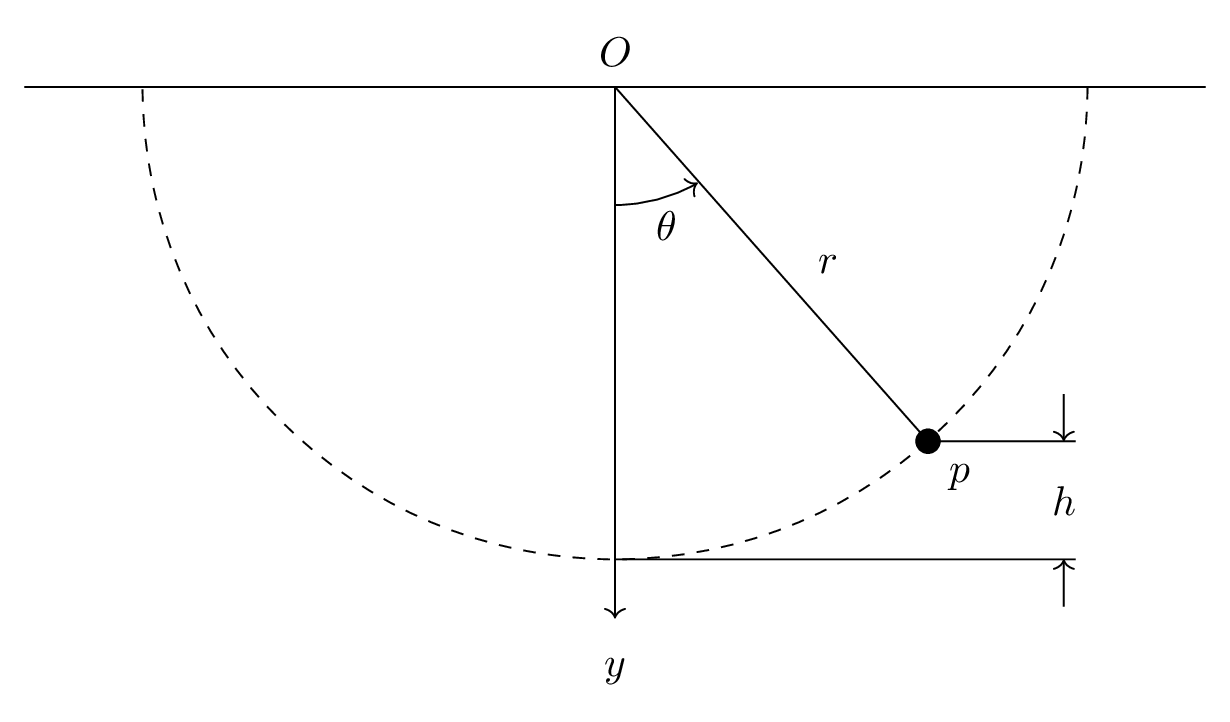
\includegraphics{Figuras/pendulo_simple}
    \caption{Esquema del péndulo simple que oscila en un arco.}
    \label{fig:figura_pendulo_simple}
\end{figure}
\end{frame}
\begin{frame}
\frametitle{Organizando el problema}
Usando el eje coordenado, vemos que el ángulo polar $\theta$ varía de $-\pi/2$ a $\pi/2$, mientras que la coordenada radial $r = Op$ permanece constante.
\end{frame}
\begin{frame}
\frametitle{Organizando el problema}
Sea $g$ la aceleración debida a la gravedad y $W$ el peso del péndulo $p$.
\\
\bigskip
\pause
La energía potencial de $p$ en $\theta = 0$ es cero. Por lo que el valor de la energía potencial en cualquier instante, es el producto de $W$ por la altura $h$:
\begin{align*}
P = W (r - r \, \cos \theta)
\end{align*}
\end{frame}
\begin{frame}
\frametitle{Organizando el problema}
Mientras que la energía cinética viene dada por
\begin{align*}
K = \dfrac{m \, v^{2}}{2} = \dfrac{1}{2} \, \dfrac{W}{g} \left( r \, \dv{\theta}{t} \right)^{2}
\end{align*}
Como el péndulo está oscilando, la energía total es constante: $P + K = C$.
\end{frame}
\begin{frame}
\frametitle{Organizando el problema}
Lo que nos permite expresar una ecuación diferencial del movimiento:
\begin{align*}
W \, r (1 - \cos \theta) + \dfrac{1}{2} \dfrac{W}{g} \left( r \dv{\theta}{t} \right)^{2} = C
\end{align*}
\end{frame}
\begin{frame}
\frametitle{Condiciones para la ec. diferencial}
Para calcular $C$ tomamos el tiempo $t = 0$ cuando $\theta = \pi/2$, vemos que el péndulo está en reposo, por lo que $\dv*{\theta}{t} = 0$, cuando $t = 0$ y $\theta = \pi/2$.
\end{frame}
\begin{frame}
\frametitle{Ecuación de movimiento}
De esta manera $C = W \, r$ y la ecuación de movimiento resulta
\begin{align*}
\dfrac{r}{2 \, g} \left( \dv{\theta}{t} \right)^{2} - \cos \theta = 0
\end{align*}
\end{frame}
\begin{frame}
\frametitle{Consideración}
Como $p$ está oscilando de un lado a otro, $\dv*{\theta}{t}$ es en ocasiones positiva y en otras negativa; podemos estimar el período $T$, calculando el tiempo que tarda de ir de $\theta=0$ a $\theta=\pi/2$, para luego multiplicar el resultado por $4$.
\\
\bigskip
\pause
De esta manera podemos usar la raíz positiva para resolver la ecuación de $\dv*{\theta}{t}$.
\end{frame}
\begin{frame}
\frametitle{Resolviendo la ecuación diferencial}
Entonces tenemos
\begin{align*}
\sqrt{\dfrac{r}{2 \, g}} \, \dv{\theta}{t} &= \cos^{1/2} \theta \dd{t} = \\[1em]
\dd{t} &= \sqrt{\dfrac{r}{2 \, g}} \, \dv{\theta}{t} \cos^{-1/2} \theta \dd{\theta} = \\[1em]
T &= 4 \, \sqrt{\dfrac{r}{2 \, g}} \, \int_{0}^{\pi/2} \cos^{-1/2} \theta \dd{\theta} = \\[1em]
\end{align*}
\end{frame}
\begin{frame}
\frametitle{Resolviendo la ecuación diferencial}
Entonces tenemos
\begin{align*}
&= 2 \, \sqrt{\dfrac{r}{2 \, g}} \, \int_{0}^{\pi/2} 2 \, \sin^{0} \theta \, \cos^{-1/2} \theta \dd{\theta} = \\[0.8em]
&= \sqrt{\dfrac{2 \, r}{g}} \, B \left( \dfrac{1}{2}, \dfrac{1}{4} \right) = \\[0.8em]
&= \sqrt{\dfrac{2 \, r}{g}} \, \dfrac{\Gamma \left(\dfrac{1}{2} \right) \, \Gamma \left(\dfrac{1}{4} \right)}{\Gamma \left(\dfrac{3}{4} \right)} = 
\end{align*}
\end{frame}
\begin{frame}
\frametitle{Resolviendo la ecuación diferencial}
\begin{align*}
T = \sqrt{\dfrac{2 \, r}{g}} \, \dfrac{\Gamma \left(\dfrac{1}{2} \right) \, 4 \, \Gamma \left(\dfrac{5}{4} \right)}{\dfrac{4}{3} \, \Gamma \left(\dfrac{7}{4} \right)}
\end{align*}
Lo que nos falta es un paso: calcular los valores de la función Gamma.
\end{frame}
\begin{frame}
\frametitle{Solución al problema}
Usando los valores para la función Gamma, se concluye que
\begin{align*}
T \cong 7.416 \sqrt{\dfrac{r}{g}}
\end{align*}
\pause
\fontsize{12}{12}\selectfont
Considera que se han omitido pasos en el desarrollo, pero en tus ejercicios deberán de estar lo más completo y detallados posible.
\end{frame}
\section{Ejercicios a cuenta}
\frame[allowframebreaks]{\tableofcontents[currentsection, hideothersubsections]}
\begin{frame}
\frametitle{Ejercicios a cuenta}
Para que puedas repasar lo revisado para las funciones Gamma y Beta, se presentan dos ejercicios.
\\
\bigskip
Recuerda que debe de haber una demostración de la fórmula o expresión que ocupes tanto para la función Gamma y/o Beta que requieras.
\end{frame}   
\subsection{Ejercicio 1}
\begin{frame}
\frametitle{E1: Distribución tipo Maxwell}
En una distribución tipo Maxwell la fracción de partículas moviéndose con velocidad $v$ y $v +\dd{v}$ es
\begin{align*}
\dfrac{\dd{N}}{N} = 4 \, \pi \left( \dfrac{m}{2 \, \pi \, k \, T} \right)^{3/2} \: \exp \left( - \dfrac{m \, v^{2}}{2 \, k \, T} \right) \: v^{2} \dd{v}
\end{align*}
donde $N$ es el número total de partículas. 
\end{frame}
\begin{frame}
\frametitle{E1: Distribución tipo Maxwell}
El promedio o valor esperado de $v^{n}$ se define como $\displaystyle \expval{v^{n}} = N^{-1} \int v^{n} \dd{N}$.
\\
\bigskip
\pause
Demostrar que:
\begin{align*}
\expval{v^{n}} = \left( \dfrac{2 \, k \, T}{m} \right)^{n/2} \dfrac{\left( \dfrac{n + 1}{2} \right) !} { \left( \dfrac{1}{2} \right) !}
\end{align*}
\end{frame}
\subsection{Ejercicio 2}
\begin{frame}
\frametitle{E2: Partícula en una cicloide}
\begin{wrapfigure}{r}{0.5\textwidth}
    \centering
    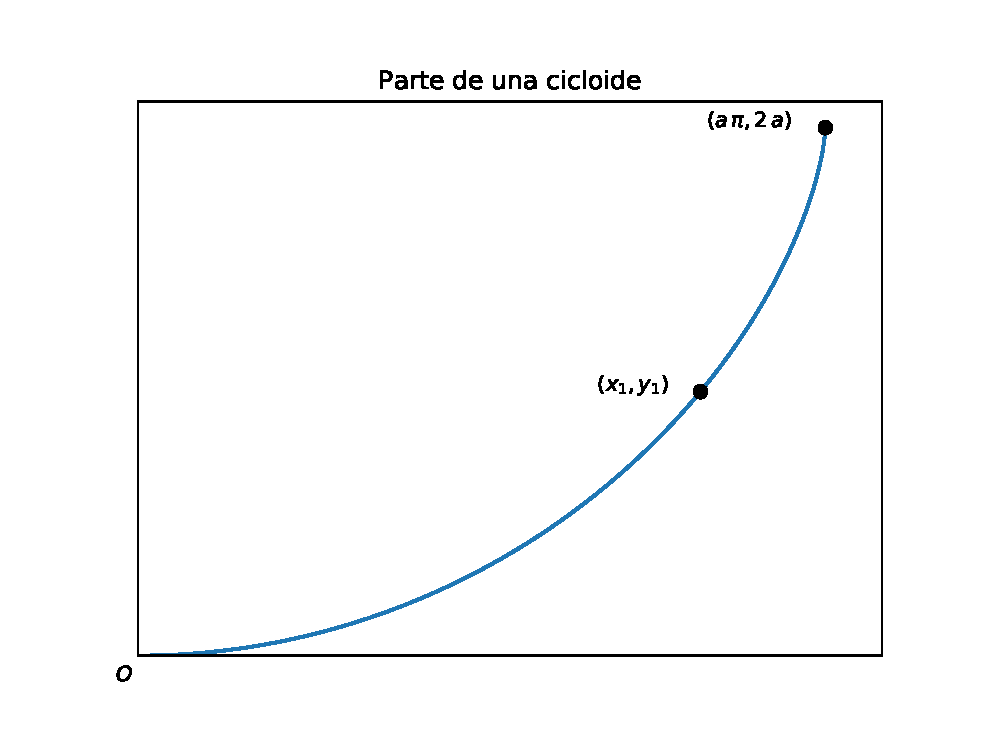
\includegraphics[width=0.5\textwidth]{Imagenes/plot_cicloide.eps}
    \caption{Una partícula deslizándose sobre una cicloide.}
    \label{fig:figura_cicloide}
\end{wrapfigure}
Se muestra en la figura (\ref{fig:figura_cicloide}) parte de una cicloide cuyas ecuaciones paramétricas son
\begin{align*}
x &= a (\theta + \sin \theta) \\[0.5em]
y &= a (1 - \cos \theta)
\end{align*}
\end{frame}
\begin{frame}
\frametitle{E2: Partícula en una cicloide}
Demuestra que el tiempo que tarda una partícula para deslizarse sin fricción a lo largo de la curva desde el punto $(x_{1}, y_{1})$ hasta el origen, está dado por
\begin{align*}
t = \sqrt{\dfrac{a}{g}} \, \int_{0}^{y_{1}} \dfrac{\dd{y}}{\sqrt{y \, (y_{1}- y)}}
\end{align*}
\end{frame}
\begin{frame}
\frametitle{E2: Partícula en una cicloide}
Sugerencia: Demuestra que la longitud del elemento de arco es $\dd{s} = \sqrt{2a/y} \dd{y}$.
\\
\bigskip
Evalúa la integral para demostrar que el tiempo es independiente de la posición inicial $y_{1}$.
\end{frame}
\end{document}